\documentclass{scrartcl}
\usepackage[utf8]{inputenc}
\usepackage[german]{babel}
\usepackage{lmodern}
\usepackage{graphicx}
\usepackage{setspace}
\usepackage{environ}
\usepackage{lipsum}
\usepackage{color}
\usepackage{setspace}
\usepackage{enumitem}
\usepackage{booktabs}
\usepackage{tabularx}
\newcolumntype{s}{>{\footnotesize}X}
\usepackage{longtable}
\usepackage{ltxtable}
\usepackage{pdflscape}
\usepackage{caption}
\captionsetup[longtable]{font={scriptsize},position=top,skip=0.5em}
\usepackage{url} 
\usepackage{float}
\setlist{leftmargin=*, label=-, nosep}
%
\usepackage[a4paper]{geometry} 
\geometry{top=25mm,left=25mm ,right=25mm, bottom=3cm} 
%\usepackage[babel,german=quotes]{csquotes}
%
% Pfad der Abbildungen
\graphicspath{ {../figures/} }
%
\setlength{\footheight}{50mm}
%\ifoot{\footnotesize  Quelle: Biologie heute 7/8, Schroedel 2006\\ Letzte Änderung: \today}
%\ofoot{Seite Nr. \luecke{1cm}}
%\ohead{Datum: \today}
%
% ----------
% ÜBERSHRIFT
% ----------
\newcommand{\Ueberschrift}[2]{
	\vskip 1.em
	\setlength{\tabcolsep}{0mm} % kein Innenrand bei Spaleten
	\begin{tabularx}{\linewidth}{lXr}
	{\Large\textbf{\textsf{#1}}} & &
	\includegraphics[scale=0.2]{#2}\\ % Logo rechtsbündig
	\hline
	\end{tabularx}
	% Spaltenabstand zurücksetzen
	\setlength{\tabcolsep}{6pt} 
}
% ----------
% HINWEISBOX
% ----------
\NewEnviron{hinweisbox}[2]{%
\par
\vspace{1em}
\noindent
\begin{tikzpicture}[]
	\node[rectangle,minimum width=1.0\textwidth, inner sep=0pt] (m) {
		\begin{minipage}{\textwidth}
			\dimen0\linewidth
			\advance\dimen0 by -3.0em
    			\vskip .8em \hspace{1em}
    			\parbox{\the\dimen0}{
        			\BODY\vskip .5em}%			
		\end{minipage}
		};
	\draw[#2, very thick, rounded corners, color=#1] (m.south west) rectangle (m.north east);
\end{tikzpicture}
}
%
% =======================
% Abbildungstext anpassen
% =======================
\usepackage[font={small}, labelfont=bf,figurename=Abb.]{caption}
%
% ----------
% AUFGABENBOX
% ----------
\NewEnviron{aufgabenbox}[2]{%
\par
\vspace{1em}
\noindent
\begin{tikzpicture}[]
	\node[rectangle,minimum width=1.0\textwidth, inner sep=0pt] (m) {
		\begin{minipage}{\textwidth}
			\dimen0\linewidth
			\advance\dimen0 by -3.0em
    			\vskip .8em \hspace{1em}
    			\parbox{\the\dimen0}{
        			\BODY\vskip .5em}%			
		\end{minipage}
		};
	\draw[solid, thin, color=black] (m.south west) rectangle (m.north east);
\end{tikzpicture}
}
%
% =====================================
% Litteraturverzeichnis und son kram...
% =====================================
\usepackage{url}
\usepackage[hidelinks]{hyperref}
% BibLaTeX
\usepackage[
style=authoryear-icomp,    % Zitierstil authoryear-icomp authoryear,natbib=true
isbn=false,                % ISBN nicht anzeigen, gleiches geht mit nahezu allen anderen Feldern
pagetracker=true,          % ebd. bei wiederholten Angaben (false=ausgeschaltet, page=Seite, spread=Doppelseite, true=automatisch)
maxbibnames=50,            % maximale Namen, die im Literaturverzeichnis angezeigt werden (ich wollte alle)
maxcitenames=2,            % maximale Namen, die im Text angezeigt werden, ab 4 wird u.a. nach den ersten Autor angezeigt
autocite=inline,           % regelt Aussehen für \autocite (inline=\parancite)
block=space,               % kleiner horizontaler Platz zwischen den Feldern
backref=false,              % Seiten anzeigen, auf denen die Referenz vorkommt
backrefstyle=three+,       % fasst Seiten zusammen, z.B. S. 2f, 6ff, 7-10
date=short,                % Datumsformat
]{biblatex}
\setlength{\bibitemsep}{1em}     % Abstand zwischen den Literaturangaben
\setlength{\bibhang}{2em}        % Einzug nach jeweils erster Zeile
% Heading Literaturverzeichnis anpassen
%\defbibheading{lit}{\part*{Literaturverzeichnis}
%	\markboth{\MakeUppercase{\refname}}{\MakeUppercase{\refname}}
%}
\bibliography{bib.bib}
%
% ----------
% StickyNote
% ----------
%\usepackage{xparse}
\usepackage{fancypar}
\usetikzlibrary{shadows}
\definecolor{myyellow}{RGB}{242,226,149}
\makeatletter
\pgfdeclareshape{note}{
\inheritsavedanchors[from=rectangle] % this is nearly a rectangle
\inheritanchorborder[from=rectangle]
\inheritanchor[from=rectangle]{center}
\inheritanchor[from=rectangle]{north}
\inheritanchor[from=rectangle]{south}
\inheritanchor[from=rectangle]{west}
\inheritanchor[from=rectangle]{east}
% ... and possibly more
\backgroundpath{% this is new
% store lower right in xa/ya and upper right in xb/yb
\southwest \pgf@xa=\pgf@x \pgf@ya=\pgf@y
\northeast \pgf@xb=\pgf@x \pgf@yb=\pgf@y
% compute corner of ‘‘flipped page’’
\pgf@xc=\pgf@xb \advance\pgf@xc by-10pt % this should be a parameter
\pgf@yc=\pgf@yb \advance\pgf@yc by-10pt
% construct main path
\pgfpathmoveto{\pgfpoint{\pgf@xa}{\pgf@ya}}
\pgfpathlineto{\pgfpoint{\pgf@xa}{\pgf@yb}}
\pgfpathlineto{\pgfpoint{\pgf@xc}{\pgf@yb}}
\pgfpathlineto{\pgfpoint{\pgf@xb}{\pgf@yc}}
\pgfpathlineto{\pgfpoint{\pgf@xb}{\pgf@ya}}
\pgfpathclose
% add little corner
\pgfpathmoveto{\pgfpoint{\pgf@xc}{\pgf@yb}}
\pgfpathlineto{\pgfpoint{\pgf@xc}{\pgf@yc}}
\pgfpathlineto{\pgfpoint{\pgf@xb}{\pgf@yc}}
\pgfpathlineto{\pgfpoint{\pgf@xc}{\pgf@yc}}
}
}
\makeatother
%\setlist{leftmargin=*,itemsep=4pt,parsep=0pt}
%\renewcommand{\labelitemi}{-}
%
\NewDocumentCommand\StickyNote{O{6cm}mO{6cm}O{0}}{%
\begin{tikzpicture}
\node[
note,
draw,
drop shadow={
  shadow xshift=2pt,
  shadow yshift=-4pt
},
inner xsep=7pt,
fill=myyellow,
rotate=#4,
inner ysep=10pt
] {\parbox[t][#1][c]{#3}{#2}};
\end{tikzpicture}%
}

\NewDocumentCommand\StickyNotePi{O{6cm}mO{6cm}O{0}}{%
\begin{tikzpicture}
\node[
note,
draw,
fill=myyellow,
inner xsep=10pt,
rotate=#4,
inner ysep=0pt,
text depth=\the\dimexpr#1+2.5ex\relax
] {\parbox[t][#1][c]{#3}{#2}};
\end{tikzpicture}%
}
%
% -----------
% Schriftstil
% -----------
%\renewcommand\familydefault{\sfdefault}
\newenvironment{uvp}{%
	\begin{longtable}{>{\footnotesize}p{2cm}ss>{\footnotesize}p{3cm}}%
		% Caption
		% #######
		\caption{%
        	\scriptsize Unterrichtsverlaufplan.%
        		Abk.: SuS: Schülerinnen und Schüler, AB: Arbeitsblatt.%
        		} \\[1em] % 
		%
		% Header (nur) auf der ersten Seite  
		% #################################          
        \toprule%
        \textbf{Phase/Zeit/\newline Dauer} & \textbf{Geplantes Verhalten der Lehrkraft/\textit{Leitimpulse}} &% 
        	\textbf{Antizipierte Aktivitäten der SuS} &% 
        \textbf{Sozialform/Medien/\newline Materialien}  \\ \midrule% 			
        \endfirsthead%
        %
        % Header auf den Folgeseiten
        % ##########################
        \caption{(Fortzsetzung)}\\ \\%
   		\toprule%
        \textbf{Phase/Zeit/\newline Dauer} &\textbf{Geplantes Verhalten der Lehrkraft/\textit{Leitimpulse}} &% 
        	\textbf{Antizipierte Aktivitäten der SuS}  &% 
        \textbf{Sozialform/Medien/\newline Materialien}  \\ \midrule% 
        \endhead%
		%        
        % Bei Seitenwechsel Tabelle mit einer Linie abschließen
		% #####################################################        
        \bottomrule \addlinespace[0.5em] \multicolumn{4}{c}{(\footnotesize Fortsetzung auf der nächsten Seite)} \\% 
        \endfoot%
		%		
		\bottomrule %
		\endlastfoot%        	

	}{\end{longtable}}%

\newcommand{\Einstieg}[5]{%
	\textbf{Einstieg} \newline #1 \newline\textcolor{red}{#2}  & #3 & #4  & #5\\ \addlinespace[.5em]
}
\newcommand{\Erarbeitung}[5]{%
	 \textbf{Erarbeitung} \newline #1 \newline\textcolor{red}{#2} & #3 & #4  & #5\\ \addlinespace[.5em]
}
\newcommand{\Sicherung}[5]{%
	 \textbf{Sicherung} \newline #1 \newline\textcolor{red}{#2} & #3 & #4  & #5\\ \addlinespace[.5em]
}
\newcommand{\Gelenk}[1]{%
	\midrule
	\multicolumn{4}{p{.95\columnwidth}}{\small \textbf{Gelenkstelle:} #1}\\ \midrule% \addlinespace[.5em]
}
\usepackage{xcolor}
\usepackage{colortbl}
\usepackage{rotating}
\usepackage[final]{pdfpages}
\titlehead{\centering 5. SPS Steglitz-Zehlendorf, Fr. Grammlich \hfill Berlin, 28. Mai 2018}
\title{Unterrichtspraktische Prüfung im Rahmen des zweiten Staatsexamens für das Lehramt an Gymnasien und Integrierten Sekundarschulen}
\subtitle{Kompetenzorientierter Unterrichtsentwurf zur Staatsprüfung im Fach Informatik}
%\author{vorgelegt von: Christoph van Heteren-Frese}
%\date{28. Mai 2018}
%
\begin{document}
% ##################################################################################################
% TITELSEITE
%
\pagenumbering{gobble}
\onehalfspace
\noindent
Studienreferendar: Christoph van Heteren-Frese \hfill Berlin, den 28. Mai 2018 \\
5. SPS Steglitz-Zehlendorf / Frau Gramlich \\
Schadow Gymnasium (06Y01)\\
Lerngruppe: in-Z2\\
Zeit: 8:45 Uhr -- 9:30 Uhr\\
Raum: II-206 \\
\onehalfspace
\begin{center}
\LARGE{\textsf{\textbf{Unterrichtspraktische Prüfung im Rahmen des zweiten Staatsexamens für das Lehramt an Gymnasien und Integrierten Sekundarschulen}}}
\par\vspace*{1cm}
\Large{\textsf{\textbf{Entwurf einer Unterrichtsstunde im Fach Informatik}}}
\par\vspace*{1cm}
\large{\textsf{\textbf{Thema der Unterrichtsreihe:}\\ Verschlüsselung im Mobilfunknetz}}
\par\vspace*{1cm}
\large{\textsf{\textbf{Thema der Stunde:}\\ Sicherer Schlüsselaustausch durch Falltürfunktionen}}
\end{center}
%\vspace*{-4em}
\begin{flushleft}
\onehalfspacing
\vspace*{3em} 
\par
\textbf{Prüfungskommission:} \newline
Prüfungsvorsitz: Fr. Spring\newline
Fachseminarleiterin Informatik: Fr. Thalemann\newline
Fachseminarleiterin Biologie: Fr.Jahn \newline
Schulleiter: Hr. Krenz 
\par\vspace*{2cm}
Berlin, den 28. Mai 2018 \hspace{.5cm} Unterschrift:\underline{\hspace{6cm}}\\ 
\end{flushleft}
%
% ##################################################################################################
\newpage
\pagenumbering{arabic}
\setcounter{page}{1}
\section{Thema der Lehr- und Lernprozesse}
\subsection{Thema der Unterrichtsreihe}
Thema der Unterrichtsreihe ist  Verschlüsselung im Mobilfunknetz.
%
\subsection{Darstellung der Unterrichtsreihe}
Die Unterrichtsreihe kombiniert Teile eines Unterrichtsmodells zum Mobilfunknetz der Arbeitsgruppe \textit{Didaktik der Informatik} (DDI) der Freien Universität Berlin (\citeyear{agddifreieuniversitatberlin_2015}) mit Auszügen der Reihe \glqq \textit{E-Mail (nur?) für Dich}\grqq\ von \textcite{gramm_2011}. Es werden u.a. die verbindlichen Inhalte Vertraulichkeit und Authentizität, die im Berliner Rahmenlehrplan im Themenfeld \textit{Informatik, Mensch und Gesellschaft} genannt werden, behandelt \parencite[23]{sek_ii}. Fokussiert werden hier \glqq\textit{Aspekte der Datensicherheit bei der Kommunikation}\grqq\ am Beispiel einer verschlüsselten Mobilfunkverbindung \parencite[16]{sek_ii}. 
%
\subsection{Thema der Unterrichtsstunde}
\enlargethispage{1cm}
Die Unterrichtsstunde fokussiert die praktische Planung eines asymmetrischen Ver\-schlüs\-sel\-ungs\-ver\-fahr\-ens, dass mit Hilfe eines Rollenspiels auf mögliche Schwachstellen hin überprüft werden soll. 
%
\LTXtable{\linewidth}{reihenplanung}
%\begin{table}[H]
%\singlespacing
%\caption{Darstellung der Unterrichtsreihe. Abkürzungen: RLP: Rahmenlehrplan, UE: Unterrichtseinheit}
%\renewcommand{\arraystretch}{1.5}
%\small
%
%\end{table}
%
\section{Kompetenzen und Standards}
\subsection{Angestrebte längerfristige Kompetenzentwicklung}
% KOMMENTAR: Formulierung des inhaltsbezogenen, kumulativ-vernetzten Aufbaus der Kompetenzentwicklung, und zwar bezogen auf die komplette Unterrichtsreihe und die gesamte Lerngruppe
Die SuS sollen durch die Unterrichtsreihe befähigt werden naturwissenschaftliche Untersuchungen selbstständig zu planen und durchzuführen. 

Die in der vorliegenden Stunde angestrebte Förderung der Teilkompetenz ist in der Klasse bisher kaum vorhanden. Die SuS haben lediglich im Rahmen einer Einzelstunde unter Anleitung ein Experiment durchgeführt. Aufbau und die Durchführung waren vollständig vorgegeben, so dass es bisher keinen selbstständigen Planungsanteil gab. Eine Progression ist dementsprechend darin zu sehen, dass  in dieser Stunde  den SuS ein Teil der Planungsarbeit überlassen wird. Wenngleich die Versuchsplanung noch nicht gänzlich selbstständig durchgeführt wird, ist der Aufbau und die Durchführung in Teilen von den SuS selbst zu planen. Des weiteren ist eine Kompetenzentwicklung im Zuwachs praktischer Fähigkeiten (Performanz) zu sehen. Dazu zählen auch allgemeine Abseitsorganisation und Zeitmanagement.
%
%Darauf aufbauend soll in den folgenden Stunden sowohl die Bildung eigener Hypothesen als auch eine reflektierte Auswertung der Ergebnisse gefördert werden, so dass sie SuS langfristig in der Lage sind Experimente mit Kontrollen selbstständig zu planen und durchzuführen \parencite[vgl.][19]{rlpbio_2015}.
%%
\subsection{Konkretisierung der Standards für die geplanten Lehr- und Lernprozesse}
\begin{table}[H]
\small
\singlespacing
\begin{tabularx}{\textwidth}{XXX}
\toprule
\textbf{Standard(s) laut RLP} & \textbf{Stand der\newline Kompetenzentwicklung} & \textbf{Standardkonkretisierung} \\
\midrule
%Die SuS... & Die SuS... & Die SuS...\\ \addlinespace[.2em]
%++++++++++++++++++++++++++++++++++++++++++++++++++++++++++++++++++++++++++++++++++++++++++++++++++++++++++++++++++++++++
 \glqq Die Schülerinnen und Schüler können Experimente zur Überprüfung von Hypothesen nach Vorgaben planen und durchführen.\grqq\ \parencite[19]{rlpbio_2015}
 & Die Lernenden können einfache Versuche mit vorgegebenem Aufbau und vollständiger Durchführungsanleitung durch\-führen und in Teilen protokollieren.
 & 
 Die Lernenden planen einen Modellversuch zum abiotischen Faktor Temperatur mit einer geeigneten Auswertung und erstellen
 dafür Teile eines Protokolls (Skizze des Versuchsaufbaus und Struktur für die geplante Auswertung).
%%++++++++++++++++++++++++++++++++++++++++++++++++++++++++++++++++++++++++++++++++++++++++++++++++++++++++++++++++++++++++
%% MAXIMALSTANDARD
%%++++++++++++++++++++++++++++++++++++++++++++++++++++++++++++++++++++++++++++++++++++++++++++++++++++++++++++++++++++++++
%\textbf{Maximalstandard ($\star\star\star$):}\newline 
%...können 
%%++++++++++++++++++++++++++++++++++++++++++++++++++++++++++++++++++++++++++++++++++++++++++++++++++++++++++++++++++++++++
%% MITLERER STANDARD
%%++++++++++++++++++++++++++++++++++++++++++++++++++++++++++++++++++++++++++++++++++++++++++++++++++++++++++++++++++++++++
%\newline\textbf{Mittlerer Standard ($\star\star$):}\newline
%... können
%%++++++++++++++++++++++++++++++++++++++++++++++++++++++++++++++++++++++++++++++++++++++++++++++++++++++++++++++++++++++++
%% MINIMALSTANDARD
%%++++++++++++++++++++++++++++++++++++++++++++++++++++++++++++++++++++++++++++++++++++++++++++++++++++++++++++++++++++++++
%\newline\textbf{Minimalstandard  ($\star$):}\newline
%... können 
\\
\bottomrule
\end{tabularx}
\end{table}
%
\subsection{Die individuelle Kompetenzentwicklung der Lernenden}
\begin{table}[H]
\small
\singlespacing
\begin{tabularx}{\textwidth}{p{2.0cm}XXX}
\toprule
\textbf{Schüler/ Standard} & \textbf{Stand der\newline Kompetenzen\-twicklung} & \textbf{Maßnahmen zur Kompetenzförderung} & \textbf{Indikatoren des Kompetenzzuwachses} \\
\midrule
\textbf{Maximal\-standard}\newline(A-Schüler) &  \textit{z.B: Eleni, Lilith, Paul:} 
\begin{itemize}
\item arbeiten zügig und selbstständig
\item können Versuchsaufbau beschreiben und erklären
\item haben noch kein Versuchsprotokoll vollstän\-dig selbstständig erstellt 
\end{itemize}
&  wird aufgefordert Störfaktoren zu benennen und zu diskutieren
& Kann die Skizze zum Versuchsaufbau selbstständig erstellen, den Versuch exakt beschreiben und zur Dokumentation eine Tabelle und eine grafische Darstellungsform vorschlagen. Die Hinweise werden nur zur Kontrolle verwendet. Wechselwirkungen und Störfaktoren werden im Versuch berücksichtigt.\\ \addlinespace[.5em]
\midrule  \addlinespace[.5em]
\textbf{Mittlerer Standard}\newline(B-Schüler) & \textit{z.B: Lissi, Cäcilia, Mark:} 
%
\begin{itemize}
\item arbeiten größtenteils selbstständig
\item haben noch kein Versuchsprotokoll vollstän\-dig selbstständig erstellt 
\end{itemize}
  & Es werden Hinweise zum Vorgehen gegeben & Kann die Skizze zum Versuchsaufbau mit Hilfe weniger Hinweise erstellen, den Versuch mit geringen Ungenauigkeiten beschreiben und zur Dokumentation der Beobachtungen  eine Tabelle vorschlagen.\\ \addlinespace[.5em]
\midrule  \addlinespace[.5em]
\textbf{Minimal\-standard}\newline(C-Schüler) & 
\textit{z. B Len, Gregor, Piotr:}
\begin{itemize}
\item können nur bedingt selbstständig arbeiten
\item sind teilweise abgelenkt
\item haben noch kein Versuchsprotokoll vollstän\-dig selbstständig erstellt 
\end{itemize}
& Es werden Hinweise zur Aufgabenverteilung (Gruppeneinteilung), zur Arbeitsweise und zur Nutzung der Hilfsmaterialien gegeben  & kann Skizze unter Nutzung aller Hinweise erstellen und den Versuch oberflächlich, aber prinzipiell richtig beschreiben. \\
\bottomrule
\end{tabularx}
\end{table}
%
\section{Sachstrukturanalyse}
Grundlegend für die asymmetrische Kryptographie sind bestimmte Funktionen, die sich zwar leicht berechnen lassen, ihre Umkehrfunktion ohne weiteres hingegen nur sehr schwer berechnet werden kann. Diese sogenannten \textit{Einwegfunktionen} mit Falltür (kurz: Falltürfunktion) verfügen aber über eine \glqq Hintertür\grqq  . Mit Hilfe dieser \glqq Hintertür\grqq\ kann die Umkehrfunktion wiederum leicht bestimmen werden. Beispielsweise lässt sich ein Briefkasten als Falltürfunktion betrachten \parencite[vgl.][11]{gramm_2011}: Während das Einwerfen eines Briefes leicht geschieht, ist es schwer, ihn danach wieder herauszufischen – es sei denn, man hat den Schlüssel zum Briefkasten. 

Im Unterricht werden Falltürfunktionen durch Vorhängeschlösser repräsentiert. Analog zu Falltürfunktion ist das Schließen eines Schlosses durch Zudrücken sehr einfach, während das Öffnen ohne Schlüssel sehr aufwendig ist.  

In Abbildung 1 sind die fachlichen Inhalte der Sequenz im Kontext der umspannenden Reihe in Form einer Mindmap dargestellt.
\begin{figure}[H]
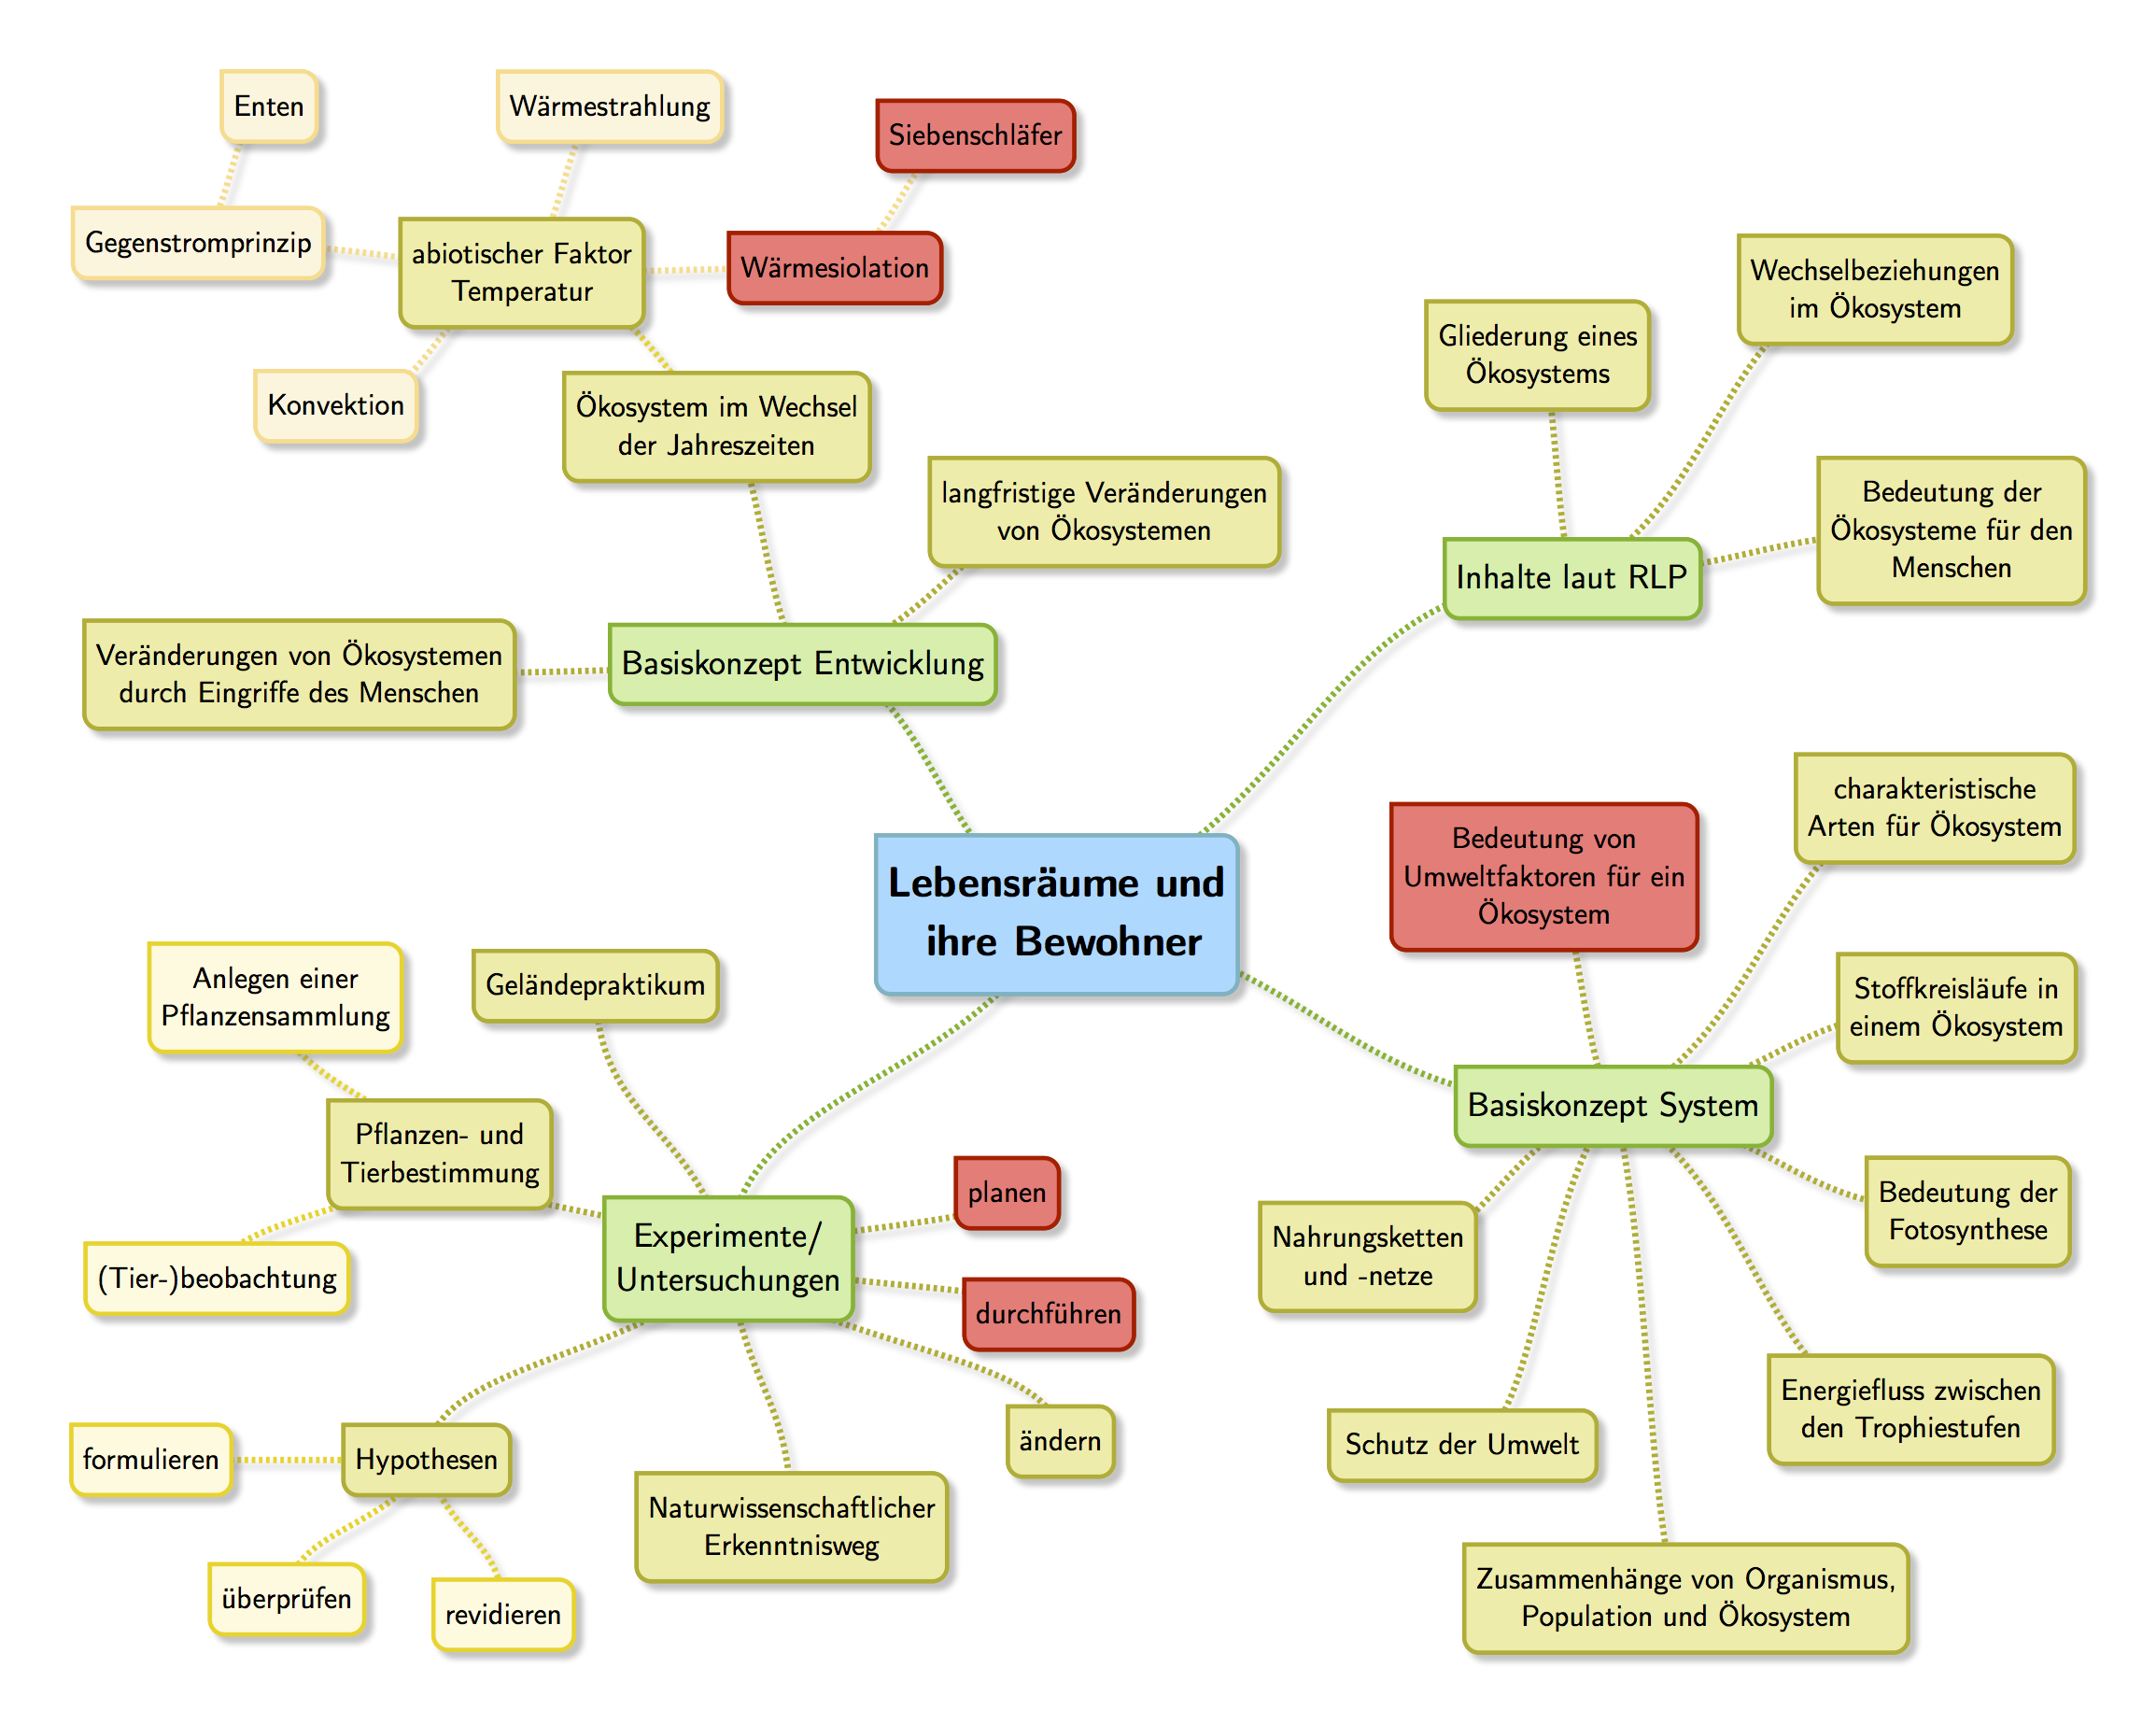
\includegraphics[width=\textwidth]{mindmap}
\caption{\small Mindmap der wichtigsten fachlichen Inhalte. Die Schlagwörter sind so angeordnet, dass der Detailgrad nach außen hin zunimmt. Inhalte der vorliegenden Stunde sind rot eingefärbt.}
\end{figure}
%
\begin{singlespacing}
\section{Begründung der Lehr- und Lernstruktur}
Ein Sachverhalt kann nach Bruner auf drei verschiedene Arten dargestellt werden: \textit{enaktiv} (d.h. handelnd), \textit{ikonisch} (d.h. bildlich) oder \textit{symbolisch}, (d.h. verbal oder formal) \parencite[49]{brunner_1974}. 
Im Sinne eines nachhaltigen Lernens sollten im Unterricht möglichst alle drei Formen genutzt werden, da sie zusammen kohärente mentale Repräsentationen ermöglichen \parencite[56]{kiper_2006}. Dabei sollte auf den Transfer zwischen den drei Repräsentationsmodi besonderer Wert gelegt werden.
\begin{landscape}
\enlargethispage{2cm}
\LTXtable{\linewidth}{Lernstruktur}
\end{landscape}
\newpage
%
\section{Unterrichtsverlaufsplan}
\LTXtable{\linewidth}{UVPlan}
\end{singlespacing}
%
% LITTERATURVERZEICHNIS
\renewcommand{\refname}{7 Literatur und Internetquellen}
\printbibliography[]
%
\newpage
\setcounter{section}{7}
\section{Anlagen}
\subsection{Sitzplan}
\begin{figure}[htbp]
\centering
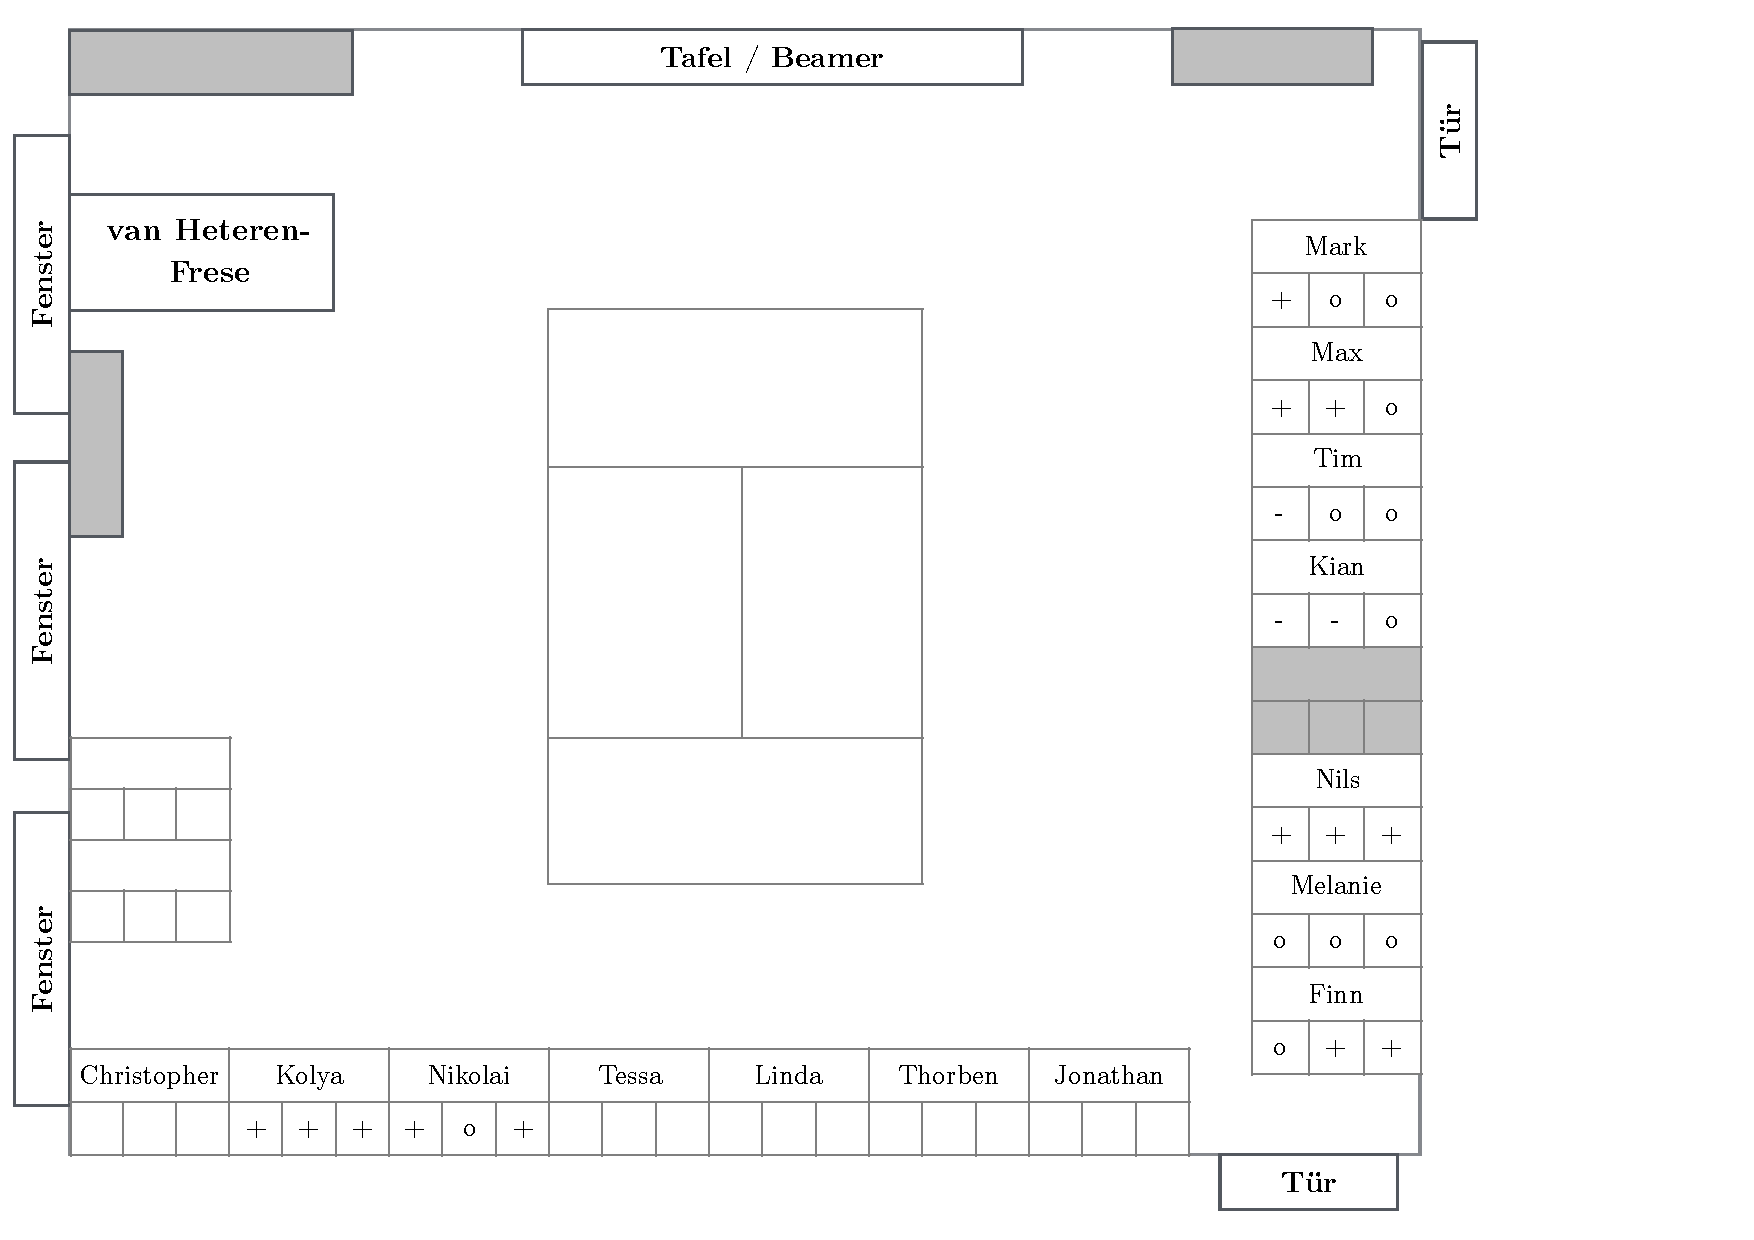
\includegraphics[width=\linewidth, clip, trim= 0cm 0.5cm 4.6cm 0cm]{Sitzplan-inz2_II206.pdf}
\caption{Sitzplan mit Leistungseinschätzung. Reihenfolge der Bewertung: \textit{Bezug zum Kompetenzschwerpunkt} $\mid$ \textit{Mitarbeit} $\mid$ \textit{Kooperation}.}
\end{figure}
%
%\enlargethispage{2cm}
\subsection{Einschätzung der Niveaus}
\begin{table}[H]
\small
\singlespacing
\centering
%\caption{Einschätzung der Niveaus}
\begin{tabularx}{\linewidth}{lXp{4cm}X}
\toprule
& \textbf{Bezug zum\newline Konpetenzschwerpunkt} & \textbf{Mitarbeit} & \textbf{Kooperation} \\
\midrule + & 
%-----------------------------------------------------------------------------------------------
kann selbstständig planen und durchführen
%-----------------------------------------------------------------------------------------------  
& regelmäßig,\newline  konstruktiv & verantwortungsvoll,\newline  zeigt Initiative \\ \addlinespace[.5em]  o &
%-----------------------------------------------------------------------------------------------
kann mit Hilfestellungen planen und durchführen
%-----------------------------------------------------------------------------------------------
& phasenweise, meist\newline  konstruktiv & erfüllt Aufgaben zielgerichtet,\newline erwartet Zuweisung \\ \addlinespace[.5em] - & 
%-----------------------------------------------------------------------------------------------
kann nur unter Anleitung und Unterstützung der Gruppe arbeiten
%-----------------------------------------------------------------------------------------------
& selten,\newline reproduzierend & ohne eigene Aktivität\\ 
\bottomrule
\end{tabularx}
\end{table}
%

\end{document}